
\begin{lem}\label{片方}
$\sharp \Sigma \ge 3$とし,$p,~q$を正規パターンとする.
正規パターンの有限集合$D$が,次の{\rm (i), (ii)}のいずれかで表されるとき,すべての$r \in D$に対して$p \{ x := r \} \preceq q$ならば,$p \{ x := xy \} \preceq q$である.

\begin{description}
\item[{\rm (i)}] $\{ ya, bc, dy \}$ $(b = a,~c \not = a,d,~b \not = d)$,
\item[{\rm (ii)}] $\{ ya, bc, dy \}$ $(b \not = a,d,~c = d,~c \not = a)$.
\end{description}
\end{lem}
\begin{proof}
$p$に変数記号が現れない場合は自明である.
したがって,$p=p_{1}xp_{2}$ ($p_{1}, p_{2}$は正規パターン, $x$は変数記号)とおく.$p \{ x := xy \} \not \preceq q$と仮定して,矛盾を導く.

\noindent\textbf{(i)}
$D=\{ ya, bc, dy \}$ $(b = a,~c \not = a,d,~b \not = d)$であるとする.
すべての$r \in D$に対して$p \{ x := r \} \preceq q$であるから
正規パターン$q$には,$ya, bc, dy$に対応する3つの長さ2の記号列が存在する.
その3つの記号列は一部を重複して現れることがあることに注意する.$D$の3つの記号列に対応する$q$の記号列の現れ方には次の3通り存在する.

\begin{description}
\item[(a)] $y_{1}a, bc, dy_{2}$,
\item[(b)] $y_{1}a, y_{2}c, dy_{3}$,
\item[(c)] $y_{1}a, by_{2}, dy_{3}$.
\end{description}

\textbf{(a)}
記号列$A,B,C$に対して,$\{ A,B,C \} = \{ y_{1}a,bc,dy_{2} \}$とおき,$q=q_{1}AwBw^{\prime}Cq_{2}$とする.
これに対して,次の式が成り立っているものとする.
\begin{align*}
(1)~& p_{1} \preceq q_{1} & (1')~& p_{2} \preceq wBw^{\prime}Cq_{2} \\
(2)~& p_{1} \preceq q_{1}Aw & (2')~& p_{2} \preceq w^{\prime}Cq_{2} \\
(3)~& p_{1} \preceq q_{1}AwBw^{\prime} & (3')~& p_{2} \preceq q_{2}
\end{align*}

$q^{\prime}_{1}=q_{1}A,~q^{\prime}_{2}=wBw^{\prime},~q^{\prime}_{3}=Cq_{2}$とおくと,(3)と(1')より,$p_{1} \preceq q^{\prime}_{1}q^{\prime}_{2},~p_{2} \preceq q^{\prime}_{2}q^{\prime}_{3}$となる.
補題\ref{補題9}より,$q^{\prime}_{2}$に変数が含まれるとき,$p \preceq q$となる.
よって,$B=y_{1}a$または,$B=dy_{2}$である場合,仮定に矛盾する.
したがって,$B=bc$である場合のみを考える.

$A=dy_{2}$とすると,(2)は$p_{1} \preceq q_{1}dy_{2}w$となる.
$p_{1}=p^{\prime}_{1}p^{\prime\prime}_{1}, p^{\prime}_{1} \preceq q_{1}d$かつ$p^{\prime\prime}_{1} \preceq y_{2}w$とおくと,(1')より,$p=p_{1}xp_{2}=p^{\prime}_{1}p^{\prime\prime}_{1}xp_{2} \preceq q_{1}dp^{\prime\prime}_{1}xwbcw^{\prime}y_{1}aq_{2}=q \{ x:=p^{\prime\prime}_{1}x \}$となり,$p=q\theta$となる.
これは仮定に矛盾する.
したがって,$A=y_{1}a,B=bc,C=dy_{2}$である場合のみ考えればよい.

以上より,記号列が重複する場合を考慮して,次の2つの場合に分けて証明する.

\begin{description}
\item[(a-1)] $q=q_{1}y_{1}awbcw^{\prime}dy_{2}q_{2}$,
\item[(a-2)] $q=q_{1}y_{1}acwdy_{2}q_{2}$ ($a=b$),
\end{description}

%$p \{ x:=ya \} \preceq q$かつ$p \{ x:=bc \} \preceq q$かつ$p \{ x:=dy \} \preceq q$ならば,
\textbf{(a-1)}
補題\ref{追加部分}の証明より,$p \{ x:= xy \} \preceq q$となる.
よって,仮定に矛盾する.

\textbf{(a-2)}
$q=q_{1}y_{1}acwdy_{2}q_{2}$ ($a=b$)とする.
この$q$に対して,次の式が成り立っているものとする.
\begin{align*}
(1)~& p_{1} \preceq q_{1} & (1')~& p_{2} \preceq cwdy_{2}q_{2} \\
(2)~& p_{1} \preceq q_{1}y_{1} & (2')~& p_{2} \preceq wdy_{2}q_{2} \\
(3)~& p_{1} \preceq q_{1}y_{1}acwdy_{2} & (3')~& p_{2} \preceq q_{2}
\end{align*}

$|w|=0$であれば,(1')と(2')より,$p_{2}$の接頭辞は$cd$かつ$d$となる.
よって,$c=d$となる.
これは,$c \not = d$であることに矛盾する.

$|w|=1$であれば,(1')と(2')より,$p_{2}$の接頭辞は$cwd$かつ$wd$となる.
よって,$w=c=d$となる.
これは,$c \not = d$であることに矛盾する.

$|w| \ge 2$であれば,(1')と(2')より,$p_{2}$の接頭辞は$cwd$かつ$wd$となる.
長さ$n$の$w$を$w_{1}w_{2}w_{3} \cdots w_{n-1}w_{n}$ $(w_{i}$ $(i=1, \ldots , n)$は定数記号$)$とする.
$cw=wd$より,$w$の接頭辞は$c$,$w$の接尾辞は$d$となる.
よって,$cw_{2}w_{3} \cdots w_{n-1}d$となる.
$cw=ccw_{2}w_{3} \cdots w_{n-1}d,~wd=cw_{2}w_{3} \cdots w_{n-1}dd$であるから,$cw=wd$より,$w_{i}=w_{i+1}$ $(i=2, \ldots , n-2)$となる.
したがって,$c=d$となる.
これは,$c \not = d$であることに矛盾する.

\textbf{(b)}の記号列を含む正規パターン$q$は,
$c \not = a$より,補題\ref{変数2つ}(i-2)に対応する記号列が現れる.
よって,$p \{ x:= xy \} \preceq q$となる.
これは,仮定に矛盾する.

\textbf{(c)}の記号列を含む正規パターン$q$は,
$b \not = d$より,補題\ref{変数2つ}(i-1)に対応する記号列が現れる.
よって,$p \{ x:= xy \} \preceq q$となる.

\noindent\textbf{(ii)}
$D=\{ ya, bc, dy \} \ (b \not = a,d,~c = d$かつ$c \not = a)$のときは,記号列$p$と$q$を逆順にすることにより,\textbf{(ii)}の場合と同様に, 仮定$p \{ x := xy \} \not\preceq q$に矛盾することを証明できる.
\end{proof}

補題\ref{追加部分},補題\ref{片方}より,次の系が得られる.

\begin{col}\label{両方}
$\sharp \Sigma \ge 3$とし,$p, q$を正規パターンとする.
正規パターンの有限集合$D= \{ ya, bc, dy \}$ $(b = a$かつ$c = d)$で表されるとき,任意の$r \in D$に対して$p \{ x := r \} \preceq q$ならば,$p \{ x := xy \} \not \preceq q$となる$q$が存在する.
\end{col}
\begin{ex}
$a,b,c,d,e$を定数記号,$x,y,y_{1},y_{2}$を変数記号とする.
$p \{ x:=xy \} \not \preceq q$となる正規パターン$p,q$を$p=eabcbcadabcbcadaxbcadadabcbcadade,~q=y_{1}abcbcadabcbcadady_{2}$ $(b = a$かつ$c = d)$とする.
\end{ex}

%\begin{figure}[H]
\begin{figure}
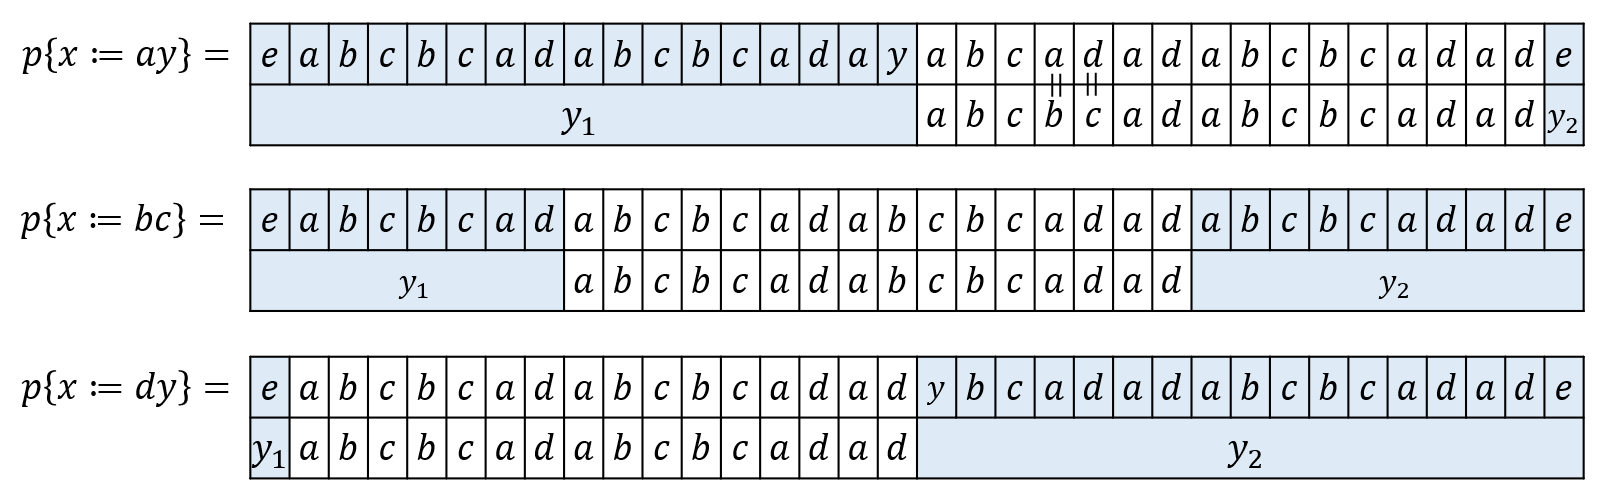
\includegraphics[width=\linewidth]{figs/Exam_b=a_c=d.png}
\vspace{-1cm}
\caption{$p$に対する代入と$q$の関係}
\label{b=aとc=dの例}
\end{figure}

このとき,図\ref{b=aとc=dの例}のように,
\begin{eqnarray*}
&p& \{ x:=ya \} \\ 
& = & (eabcbcadabcbcaday)abcadadabcbcadade\\
& = & q \{ y_{1} := eabcbcadabcbcaday_{1} \} \\
& \preceq & q,\\
&p& \{ x:=bc \}  \\
& = & (eabcbcad)abcbcadabcbcadad(abcbcadade) \\
& = & q \{ y_{1} := eabcbcad,~y_{2} := abcbcadade \} \\
& \preceq & q,\\
&p& \{ x:=dy \}  \\
& = & eabcbcadabcbcadad(ybcadadabcbcadade) \\
& = & q \{ y_{2} := y_{2}bcadadabcbcadade \} \\
& \preceq & q.
\end{eqnarray*}
となる.
これは,系\ref{両方}の条件を満たす.
\begin{comment}
\begin{lem}\label{追加補題2}
$\sharp \Sigma \ge 3$とし,$p, q$を正規パターンとする.
正規パターンの有限集合$D= \{ ya,ab,by,cd \}$ $(cd \not = ab)$で表されるとき,すべての$r \in D$に対して$p \{ x := r \} \preceq q$ならば,$p \{ x := xy \} \preceq q$である.
\end{lem}
\begin{proof}
$p$に変数記号が現れない場合は自明である.
したがって,$p=p_{1}xp_{2}$ ($p_{1}, p_{2}$は正規パターン, $x$は変数記号)とおく.$p \{ x := xy \} \not \preceq q$と仮定して,矛盾を導く.

$c \not = a$かつ$d \not = b$であるとき,系\ref{両方}より,$p \{ x:= xy \} \preceq q$となる.
これは,仮定に矛盾する.

$c \not = a$かつ$d = b$,または,$c = a$かつ$d \not = b$であるとき,補題\ref{片方}より,$p \{ x:=xy \} \preceq q$となる.
これは,仮定に矛盾する.
\end{proof} 
\end{comment}
%\begin{lem}\label{追加補題1}
%$k \ge 3$,$m \ge \sqrt{k+1}$,$\sharp \Sigma \ge k+m$,$P \in \RPatplus$,$Q \in \RPat^{k}$とする.
%すべての定数記号$a, b \in \Sigma$に対し,ある正規パターン$q \in Q$が存在し,
%$p \{ x:=ab \} \preceq q$ならば,$p \{ x:=xy \} \preceq q$となる.
%\end{lem}

\begin{lem}\label{追加補題1}
$\sharp \Sigma \ge k+2$,$p \in \RPat$,$Q \in \RPat^{k}$とする.
任意の定数記号$a, b \in \Sigma$に対し,ある正規パターン$q \in Q$が存在し,
$p \{ x:=ab \} \preceq q$ならば,$p \{ x:=xy \} \preceq q$となる.
\end{lem}
\begin{proof}
$p$に変数記号が現れない場合は自明である.
したがって,$p=p_{1}xp_{2}$ ($p_{1},p_{2}$は正規パターン,$x$は変数記号)とおく.
また,$Q=\{ q_{1}, \ldots , q_{k} \}$とする.次のように記号を定める.
\begin{align*}
& A_{i} = \{ a \in \Sigma \mid p \{ x:=ay \} \preceq q_{i},\ y\in X\},\\ 
& B_{i} = \{ b \in \Sigma \mid p \{ x:=yb \} \preceq q_{i},\ y\in X\},\\ 
%& \tilde{B}_{i} = \{ \tilde{b} \in \Sigma \mid p \{ x:=yb \} \preceq q_{i},\ y\in X\},\\ 
& A = \bigcup_{i=1}^{k}A_{i},B = \bigcup_{i=1}^{k} B_{i},\\
& \tilde{B} = \{ \tilde{b} \mid b \in B \},\\
& A^{\prime} = \Sigma\setminus A,~B^{\prime} = \Sigma\setminus B,\\
& \tilde{\Sigma} = \{ \tilde{c} \mid c \in \Sigma \},\\
& \tilde{B}^{\prime} = \{ b \mid b \in \tilde{\Sigma} \setminus \tilde{B} \}~~(i=1, \ldots , k).
\end{align*}

$p \{ x:=xy \} \not \preceq q_{i}$ \ ($i=1, \ldots , k$)と仮定する.

$k=1$のとき,$p \{ x:=a_{1}a_{i} \} \preceq q_{1}$かつ$p \{ x:=a_{2}a_{i} \} \preceq q_{1}$ ($i=1,2,3$)となる.
$p^{\prime} = p \{ x:=a_{1}y \} = p_{1}a_{1}yp_{2}$とおくと,$p \{ x:=a_{1}a_{i} \} \preceq q_{1}$より,$p^{\prime} \{ y:=a_{i} \} \preceq q_{1}$となる.
$a_{i}$は互いに異なる定数記号であるため,補題\ref{補題10}より,$p^{\prime} \preceq q_{1}$となる.
よって,$p \{ x:=a_{1}y \} \preceq q_{1}$となる.
$p \{ x:=a_{2}y \}$についても同様に考えることができ,$p \{ x:=a_{2}y \} \preceq q_{1}$となる.
したがって,$p \{ x:=a_{1}y \} \preceq q_{1}$かつ$p \{ x:=a_{2}y \} \preceq q_{1}$であるため,補題\ref{変数2つ}より,$p \{ x:= xy \} \preceq q_{1}$となる.
これは,仮定に矛盾する.

$k \ge 2$のとき,2部グラフを用いて矛盾を導く.
$G=(\Sigma,\tilde{\Sigma}; A^{\prime} \times \tilde{B}^{\prime})$
を$\Sigma$と$\tilde{\Sigma}$を部集合とし,$A^{\prime} \times \tilde{B}^{\prime}$を辺集合とする2部グラフとする.
$\Sigma$と$\tilde{\Sigma}$を部集合とし,$\tilde{E}_{i}=\{ (a, \tilde{b}) \in A^{\prime} \times \tilde{B}^{\prime} \mid p \{ x:=ab \} \preceq q_{i} \}$を辺集合とする2部グラフを$\tilde{G}_{i}=(\Sigma,\tilde{\Sigma}; \tilde{E}_{i})$とする.

$\sharp A_{i} \ge 2$または$\sharp B_{i} \ge 2$となる$i$が存在するとき,補題\ref{変数2つ}より,$p \{ x:=xy \} \preceq q_{i}$となる.
これは仮定に矛盾する.よって,任意の$i$ ($i=1, \ldots , k$)に対して,$\sharp A_{i} \le 1$かつ$\sharp B_{i} \le 1$となる.
また,$0 \le \sharp A \le k$かつ$0 \le \sharp\tilde{B} \le k$となり,$2 \le \sharp A^{\prime} \le k+2$かつ$2 \le \sharp \tilde{B}^{\prime} \le k+2$となる.
$\sharp A=k$かつ$\sharp \tilde{B}=k$である$G$を$G^{(k,~k)}$と表し,$\sharp A_{i}=1$かつ$\sharp B_{i}=1$である$\tilde{G}_{i}$を$\tilde{G}^{(1,~1)}_{i}$と表す.

$\sharp A$と$\sharp \tilde{B}$の関係を,次の3つの場合に分けて証明する.
\[
\begin{tabular}{ll}
$\textbf{(1)}$ $\sharp A=k$かつ$\sharp \tilde{B} \le k$,\\
$\textbf{(2)}$ $\sharp A = k-1$かつ$\sharp \tilde{B} \le k-1$,\\
$\textbf{(3)}$ $\sharp A \le k-2$かつ$\sharp \tilde{B} \le k-2$,
\end{tabular}
\]
\begin{figure*}
\centering
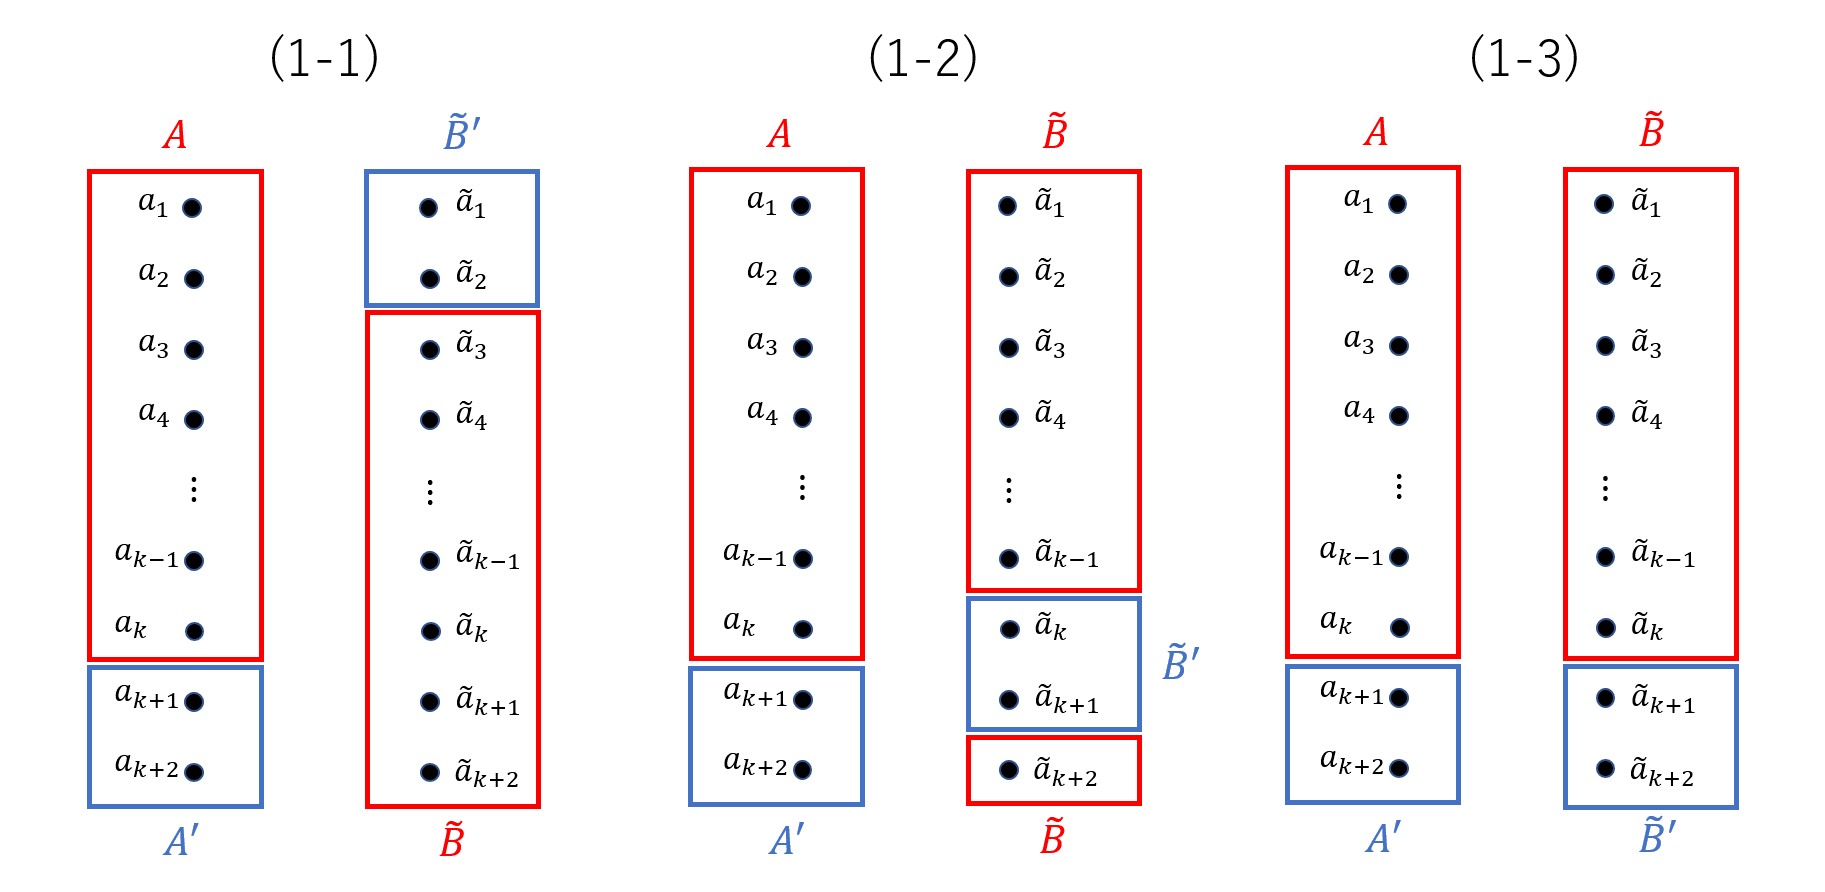
\includegraphics[width=\linewidth]{figs/ComparingBipartiteGraph.png}
\vspace{-1cm}
\caption{(1-1),(1-2),(1-3)の例}
\label{グラフ比較}
\end{figure*}

\noindent\textbf{(1)} 
$\sharp A=k$かつ$\sharp \tilde{B} \le k$であるとき,$\sharp A^{\prime}=2$かつ$\sharp \tilde{B}^{\prime} \ge 2$となる.
このとき,$G$には少なくとも$\sharp A^{\prime} \times \sharp \tilde{B}^{\prime}=2\times2=4$本の辺が含まれる.
図\ref{グラフ比較}のように,$| A^{\prime} \cap B^{\prime} |$の関係は,3種類に分けられる.
よって,以下のように,場合分けして証明する.
\[
\begin{tabular}{ll}
$\textbf{(1-1)}$ $| A^{\prime} \cap B^{\prime} | = 0$,$\textbf{(1-2)}$ $| A^{\prime} \cap B^{\prime} | = 1$,\\
$\textbf{(1-3)}$ $| A^{\prime} \cap B^{\prime} | = 2$.
\end{tabular}
\]

\textbf{(1-1)} 
$\sharp A = k$かつ$\sharp \tilde{B} = k$であるとき,
$p \{ x:=ya_{i} \} \preceq q_{i}$かつ$p \{ x:=a_{i}y \} \preceq q_{i}$ $(i=3,\ldots,k)$とし,$p \{ x:=a_{j}y \} \preceq q_{j}$かつ$p \{ x:=ya_{k+j} \} \preceq q_{j}$ $(j=1,2)$とする.

%\begin{figure}[H]
\begin{figure}  
\centering
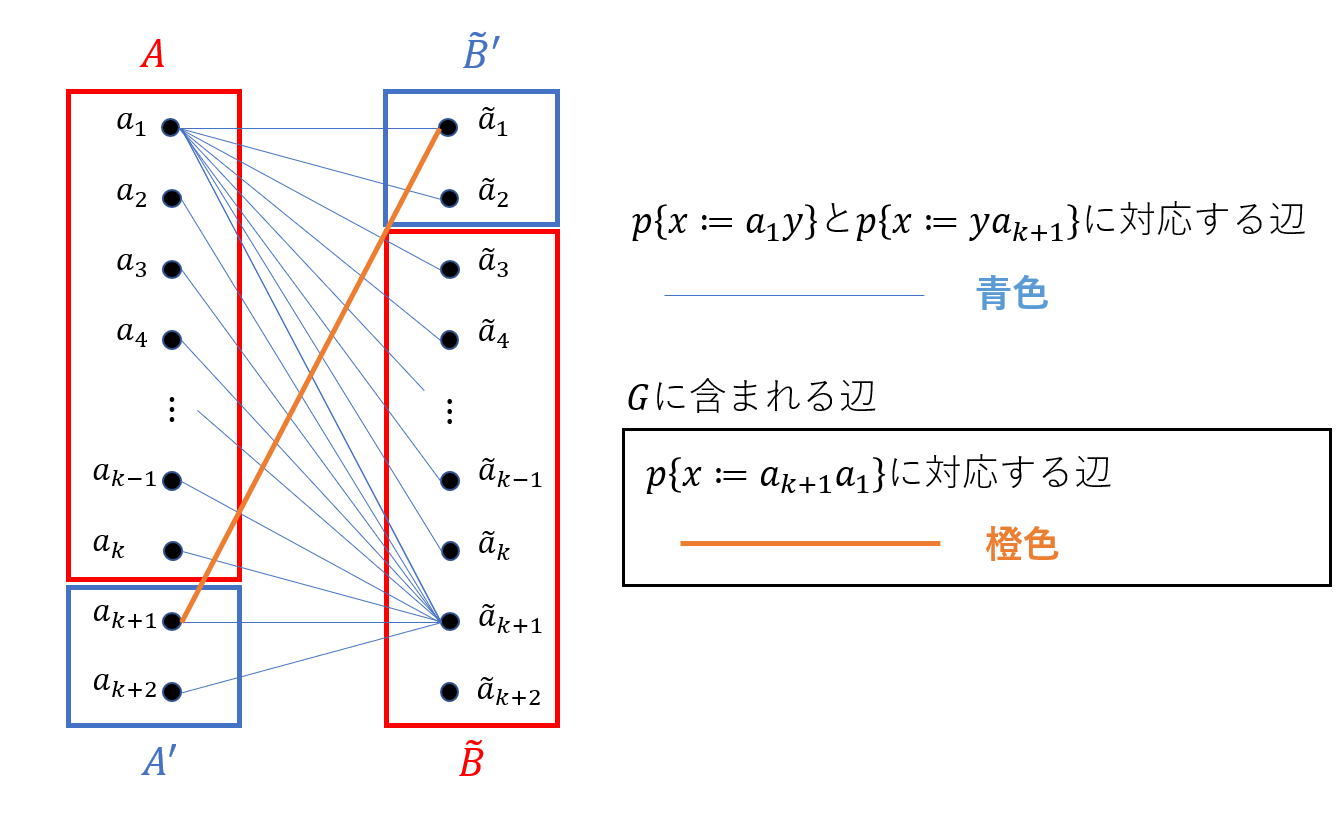
\includegraphics[width=\linewidth]{figs/Exam-BipartiteGraph-Corollary.png}
\vspace{-1cm}
\caption{系\ref{両方}の条件に当てはまるパターンにおける二分グラフの例}
\label{系との関係}
%\vspace*{-.5cm}
\end{figure}

系\ref{両方}より,$p \{ x:=a_{k+1}a_{1} \} \preceq q_{1}$(図\ref{系との関係}),$p \{ x:=a_{k+2}a_{2} \} \preceq q_{2}$となる$q_{1},~q_{2}$が考えられる.

このとき,$\tilde{G}_{1}$と$\tilde{G}_{2}$に含まれる辺はそれぞれ1本となる.
$G$に含まれる辺は,4本であるため,残り$4-2=2$本の辺は$\tilde{G}_{i}$ $(i=3, \ldots, k)$に含まれる.
すなわち,$p \{ x:=a_{k+1}a_{2} \} \preceq q_{i_{0}}$と$p \{ x:=a_{k+2}a_{1} \} \preceq q_{i_{1}}$となる$q_{i_{0}}$と$q_{i_{1}}$が存在する.
任意の$i$ $(i=3, \ldots, k)$に対して,$p \{ x:=ya_{i} \} \preceq q_{i}$かつ$p \{ x:=a_{i}y \} \preceq q_{i}$であるため,$q_{i_{0}},q_{i_{1}} \in Q \setminus \{ q_{1},q_{2} \}$より,$a_{k+1} \not = a_{i}$かつ$a_{2} \not = a_{i}$となる.
よって,補題\ref{追加部分}より,$p \{ x:=xy \} \preceq q_{i_{0}}$となり,仮定に矛盾する.

$\sharp A = k$かつ$\sharp \tilde{B} < k$であるとき,$\sharp A_{i}=1$かつ$\sharp B_{i}=0$となる$i$が存在する.

%\begin{figure}[H]
\begin{figure}
\centering
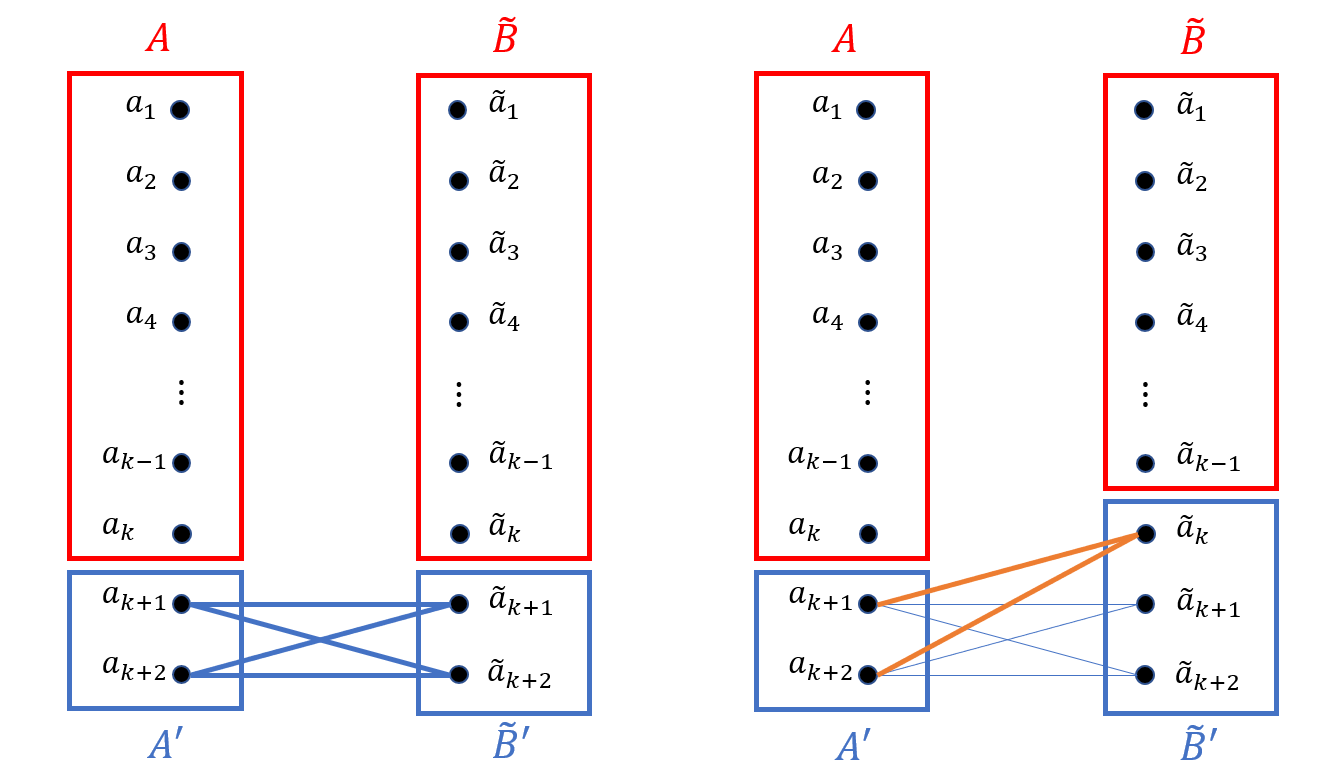
\includegraphics[width=\linewidth]{figs/BipartiteGraph-diff-ab.png}
\vspace{-1cm}
\caption{$\sharp A_{k} =1$かつ$\sharp B_{k}=1$の場合と$\sharp A_{k}=1$かつ$\sharp B_{k}=0$の場合の$G$に含まれる辺数の違い}
\label{abが異なる場合}
\end{figure}

図\ref{abが異なる場合}のように,$G^{(k,~k-1)}$に含まれる辺の本数は,$G^{(k,~k)}$と比べて,$\sharp A^{\prime}$本多くなる.
すなわち,ある$\tilde{G}^{(1,~1)}_{i}$が$\tilde{G}^{(1,~0)}_{i}$となった場合,全体の$G$に含まれる辺の本数は,$\sharp A^{\prime}$本多くなる.
このことから,$G^{(k,~k-1)}$の部分グラフ$\tilde{G}^{(1,~0)}_{i}$に含まれる辺の本数が$\sharp A^{\prime}$本以下であるとき,$G^{(k,~k)}$における結果と同様となる.
一方で,$G^{(k,~k-1)}$の部分グラフ$\tilde{G}^{(1,~0)}_{i}$に$\sharp A^{\prime}+1=2+1=3$本以上の辺が含まれるとき,$G^{(k,~k)}$における結果から変化する可能性がある.

$G^{(k,~k-2)}$の部分グラフ$\tilde{G}^{(1,~0)}_{i_{0}}$と$\tilde{G}^{(1,~0)}_{i_{1}}$が,それぞれ$3$本の辺を含むとき,以下のような例が考えられる.

\begin{ex}\label{少なくなるとき}
${G}^{(k,~k-2)}$の部分グラフ$\tilde{G}^{(1,~0)}_{k-1}$と$\tilde{G}^{(1,~0)}_{k}$に$\sharp A^{\prime}+1=2+1=3$本の辺が含まれるとき,
\begin{description}
\item[$(\mathrm{i})$] $p \{ x:= a_{i}y \} \preceq q_{i}$かつ$p \{ x:= ya_{i} \} \preceq q_{i}$ $(i=3, \ldots , k-2)$,
\item[$(\mathrm{ii})$] $p \{ x:=a_{j}y \} \preceq q_{j},~p \{ x:=ya_{k+j} \} \preceq q_{j}$かつ$p \{ x:=a_{k+j}a_{j} \} \preceq q_{j}$ $(j=1,2)$,
\item[$(\mathrm{iii})$] $p \{ x:=a_{k-1}y \} \preceq q_{k-1},~p \{ x:=a_{z}a_{k-1} \} \preceq q_{k-1}$かつ$p \{ x:=a_{1}a_{k+2} \} \preceq q_{k-1}$ \\$(z=k+1,k+2)$,
\item[$(\mathrm{iv})$] $p \{ x:=a_{k}y \} \preceq q_{k},~p \{ x:=a_{z}a_{k} \} \preceq q_{k}$かつ$p \{ x:=a_{2}a_{k+1} \} \preceq q_{k}$.
\end{description}
となる$p$と$q_{i}$ $(i=1,\ldots,k)$が存在し,$p \{ x:=xy \} \not \preceq q_{i}$となる.
\end{ex}
%例\ref{少なくなるとき}において,$G^{(k,k)}$の部分グラフ$\tilde{G}_{i},\tilde{G}_{j}$と$G^{(k,k-2)}$の部分グラフ$\tilde{G}_{i},\tilde{G}_{j}$に含まれる辺数は変わらない.
%よって,$\tilde{G}_{k-1}$と$\tilde{G}_{k}$に注目すればよい.
%$G^{(k,k)}$には$2 \times 2=4$本の辺が含まれ,$G^{(k,k-2)}$には$2 \times 4=8$本の辺が含まれる.
%$\sharp ((\tilde{A} \times \tilde{B}) \setminus E_{i})$は,$G^{(k,k)}$に含まれる辺の$\sharp (\tilde{A} \times \tilde{B})=4$本より少なくなる.
%(1)の場合,$\sharp\tilde{A} = 2$より,$\tilde{G}^{(1,0)}_{i}$に$2+1=3$本以上の辺が含まれるとき,$\sharp ((\tilde{A} \times \tilde{B}) \setminus E_{i})$は,$G^{(k,k)}$に含まれる辺の$\sharp (\tilde{A} \times \tilde{B})$本より少なくなる.
%$\tilde{G}^{(1,0)}_{k-1}$と$\tilde{G}^{(1,0)}_{k}$が,それぞれ$\sharp A^{\prime}+1$=3本の辺を持つ場合,$\tilde{G}_{i}$には辺は含まれない.
%よって,$p \{ x:=xy \} \not \preceq q_{i}$ $(i=1,\ldots,k)$となる.

%\begin{figure}[H]
\begin{figure}
\centering
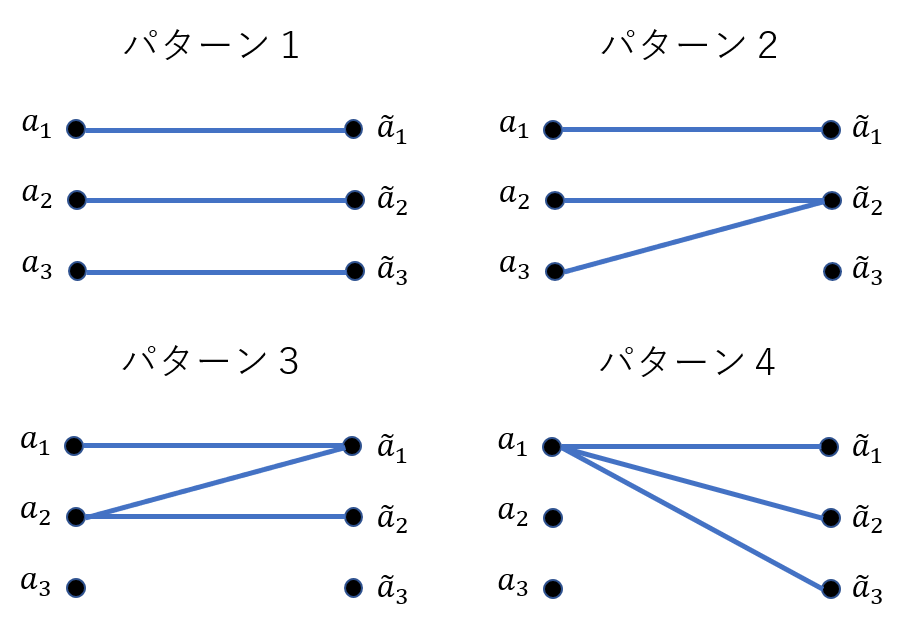
\includegraphics[width=\linewidth]{figs/BipartiteGraph-NumEdges-3.png}
\vspace*{-1cm}
\caption{辺数が3である二分グラフの例}
\label{辺3におけるパターン}
\end{figure}

図\ref{辺3におけるパターン}のように,$\tilde{G}^{(1,~0)}_{i}$に3本の辺が含まれるパターンは,4つ存在する.
パターン1の場合,補題\ref{補題14}(abc)より,$p \{ x:=xy \} \preceq q_{i}$となる.
パターン2とパターン3の場合,互いに隣接しない辺が2本存在するため,
補題\ref{補題14}(d)より,$p \{ x:=xy \} \preceq q_{i}$となる.
パターン4の場合,$p \{ x:=a_{1}a_{j} \} \preceq q_{i}$ $(j=1,2,3)$となる.
$p^{\prime} = p \{ x:=a_{1}y \} = p_{1}a_{1}yp_{2}$とおくと,$p \{ x:=a_{1}a_{j} \} \preceq q_{i}$より,$p^{\prime} \{ y:=a_{j} \} \preceq q_{i}$となる.
$a_{j}$は互いに異なる定数記号であるため,補題\ref{補題10}より,$p^{\prime} \preceq q_{i}$となり,$p \{ x:=a_{1}y \} \preceq q_{i}$となる.
これは,$A_{i}$の定義に矛盾する.
よって,$\tilde{G}^{(1,~0)}_{i}$に含まれる辺は2本以下となる.
したがって,例\ref{少なくなるとき}は,$\tilde{G}^{(1,~0)}_{k-1}$と$\tilde{G}^{(1,~0)}_{k}$に含まれる辺がそれぞれ2本以下であることに矛盾する.

以上より,$G^{(k,~k)}$において,仮定に矛盾する場合,$\sharp A=k$かつ$\sharp \tilde{B}^{\prime} < k$である場合においても,仮定に矛盾する.
(2),(3)のいずれの場合においても,$\sharp A^{\prime} > 2$であることから,同様のことが言える.

\textbf{(1-2)} 
$\sharp A = k$かつ$\sharp \tilde{B} = k$であるとき,
$p \{ x:=ya_{i} \} \preceq q_{i}$かつ$p \{ x:=a_{i}y \} \preceq q_{i}$ $(i=1,\ldots,k-1)$とし,$p \{ x:= ya_{k+2} \} \preceq q_{k}$かつ$p \{ x:= a_{k}y \} \preceq q_{k}$とする.
系\ref{両方}より,$p \{ x:=a_{k+2}a_{k} \} \preceq q_{k}$である$q_{k}$が考えられる.
このとき,$\tilde{G}_{k}$に含まれる辺は1本となる.
$G$に含まれる辺は,4本であるから,残り$4-1=3$本の辺は$\tilde{G}_{i}$ $(i=1, \ldots, k-1)$に含まれる.
すなわち,$p \{ x:=a_{k+1}a_{k+1} \} \preceq q_{i_{0}}$が存在する.
任意の$i$ $(i=1, \ldots, k-1)$に対して,$p \{ x:=ya_{i} \} \preceq q_{i}$かつ$p \{ x:=a_{i}y \} \preceq q_{i}$であるため,$q_{i_{0}} \in Q \setminus \{ q_{k} \}$より,$a_{k+1} \not = a_{i}$となる.
よって,補題\ref{追加部分}より,$p \{ x:=xy \} \preceq q_{i_{0}}$となり,仮定に矛盾する.

\textbf{(1-3)} 
$\sharp A = k$かつ$\sharp \tilde{B} = k$であるとき,
$p \{ x:=ya_{i} \} \preceq q_{i}$かつ$p \{ x:=a_{i}y \} \preceq q_{i}$ $(i=1,\ldots,k)$とする
$G$に$4$本の辺が含まれるため,$p \{ x:=a_{k+1}a_{k+1} \} \preceq q_{i_{0}}$が存在する.
よって,任意の$i$に対して,$a_{k+1} \not = a_{i}$となる.
補題\ref{追加部分}より,$p \{ x:=xy \} \preceq q_{i_{0}}$となり,仮定に矛盾する.

\begin{figure*}
\centering
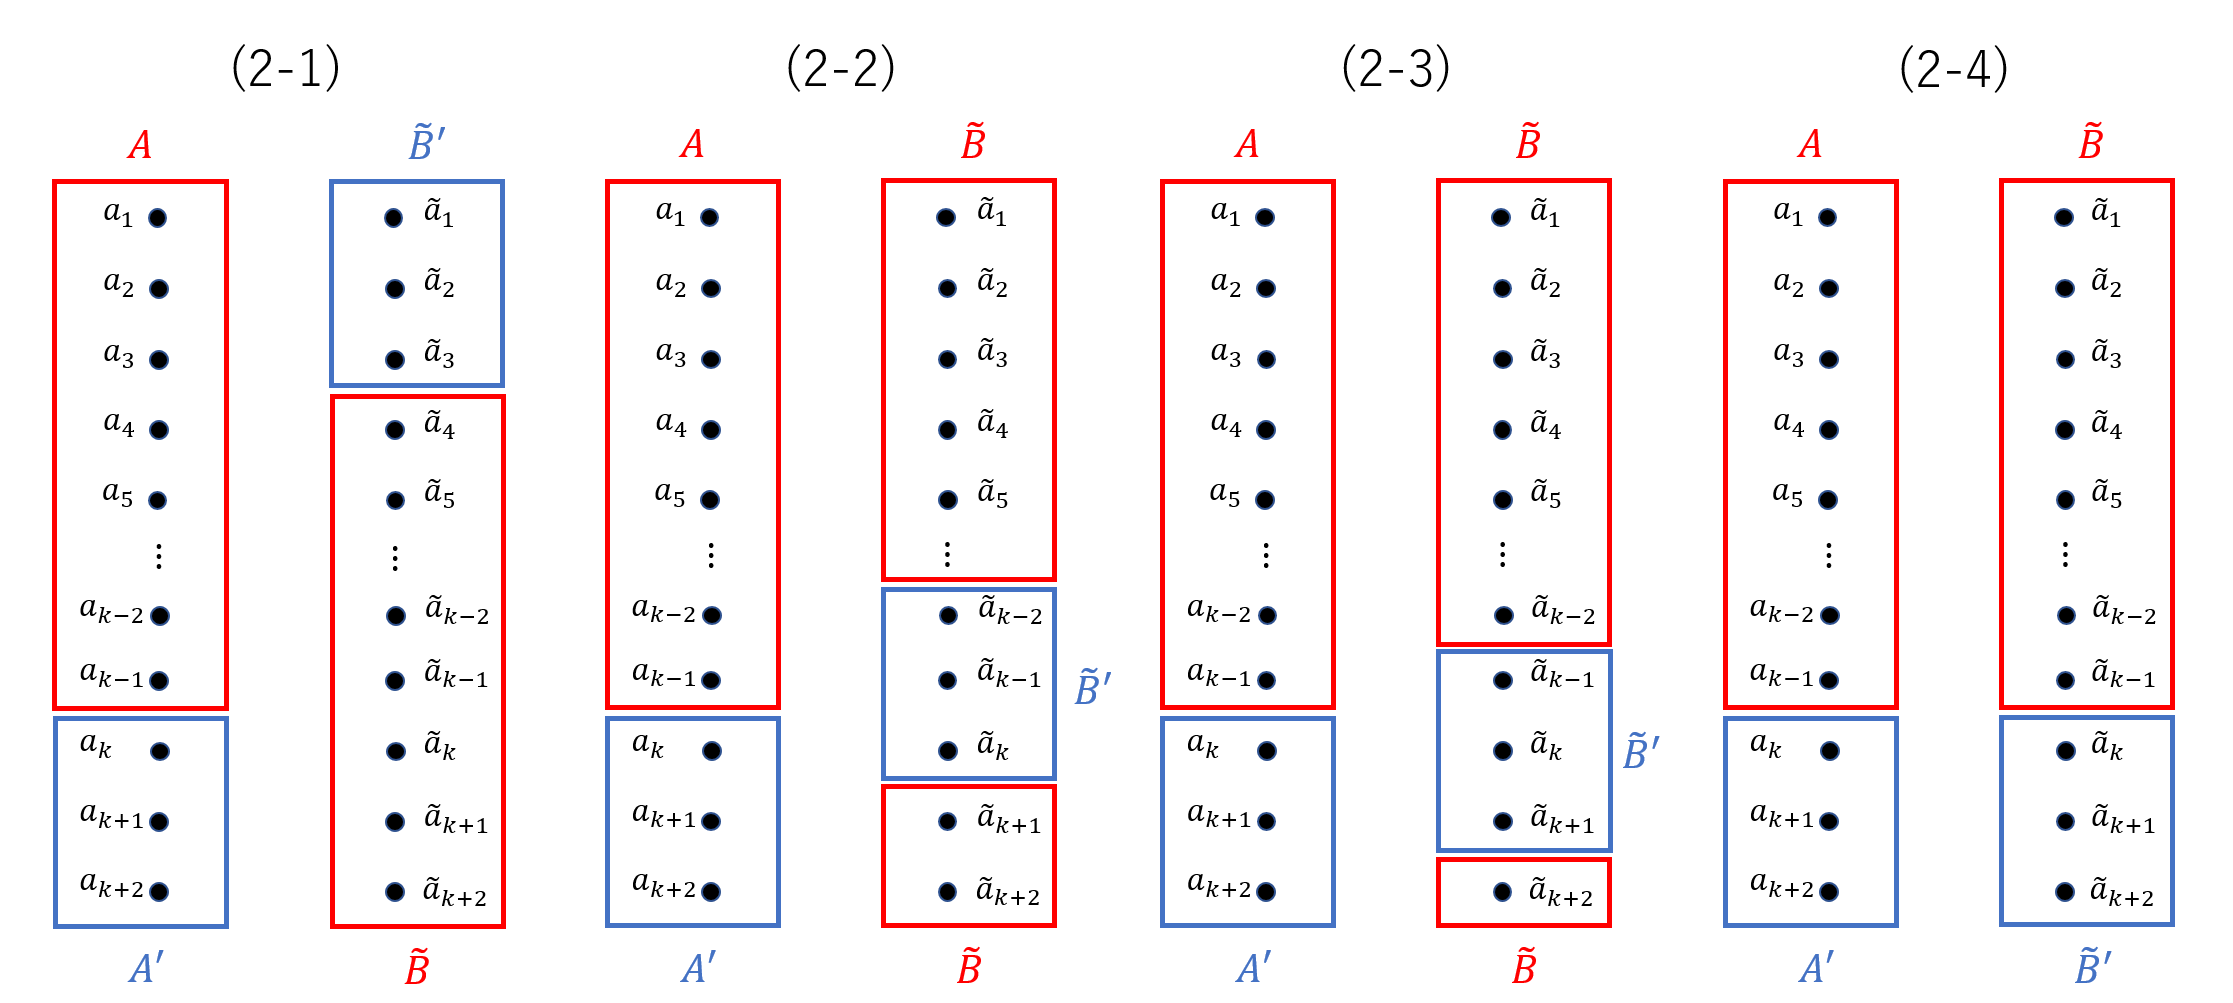
\includegraphics[width=\linewidth]{figs/Exam-Cases-(2).png}
\vspace*{-1cm}
\caption{(2-1),(2-2),(2-3),(2-4)の例}
\label{(2)におけるパターン}
\end{figure*}

\noindent\textbf{(2)} 
$\sharp A=k-1$かつ$\sharp B \le k-1$であるとき,$\sharp A^{\prime}=3$かつ$\sharp \tilde{B}^{\prime} \ge 3$となる.
$G$には少なくとも$\sharp A^{\prime} \times \sharp \tilde{B}^{\prime}=3\times3=9$本の辺が含まれる.
図\ref{(2)におけるパターン}のように,$| A^{\prime} \cap B^{\prime} |$の関係は,4種類に分けられる.よって,以下のように,場合分けして証明する.
\[
\begin{tabular}{ll}
$\textbf{(2-1)}$ $| A^{\prime} \cap B^{\prime} | = 0$,$\textbf{(2-2)}$ $| A^{\prime} \cap B^{\prime} | = 1$,\\
$\textbf{(2-3)}$ $| A^{\prime} \cap B^{\prime} | = 2$,$\textbf{(2-4)}$ $| A^{\prime} \cap B^{\prime} | = 3$.
\end{tabular}
\]

\textbf{(2-1)} 
$\sharp A=k-1$かつ$\sharp \tilde{B}=k-1$であるとき,
$p \{ x:=ya_{i} \} \preceq q_{i}$かつ$p \{ x:=a_{i}y \} \preceq q_{i}$ $(i=4, \ldots, k-1)$とし,$p \{ x:=ya_{j} \} \preceq q_{j}$かつ$p \{ x:=a_{k+j-1}y \} \preceq q_{j}$ $(j=1,2,3)$とする.
このとき,系\ref{両方}より,$p \{ x:=a_{j}a_{k+j-1} \} \preceq q_{j}$となる$q_{j}$が考えられる.
よって,$\tilde{G}_{j}$には,それぞれ1本の辺が含まれる.
$G$に含まれる辺は,9本であるから,残り$9-3=6$本の辺は$\tilde{G}_{i}$ $(i=4, \ldots, k)$に含まれる.
$\tilde{G}_{i}$ $(i=4, \ldots, k-1)$のいずれかに,辺が1本以上含まれる場合,$p \{ x:=ab \} \preceq q_{i}$ $(a \not = a_{i}$かつ$b \not = a_{i})$となる.
これは,補題\ref{追加部分}より,$p \{ x:=xy \} \preceq q_{i}$となるため,仮定に矛盾する.
よって,$\tilde{G}_{k}$には$6$本の辺が含まれる.
次数が3以上である頂点$a$が$\tilde{G}_{k}$に含まれるとき,補題\ref{補題10}より,$p \{x:=ay \} \preceq q_{k}$または$p \{ x:= ya \} \preceq q_{k}$となり,$A_{k}$または$B_{k}$の定義に矛盾する.
したがって,$\tilde{G}_{k}$に含まれる頂点の次数は2以下となる.

%\begin{figure}[H]
\begin{figure}
\centering
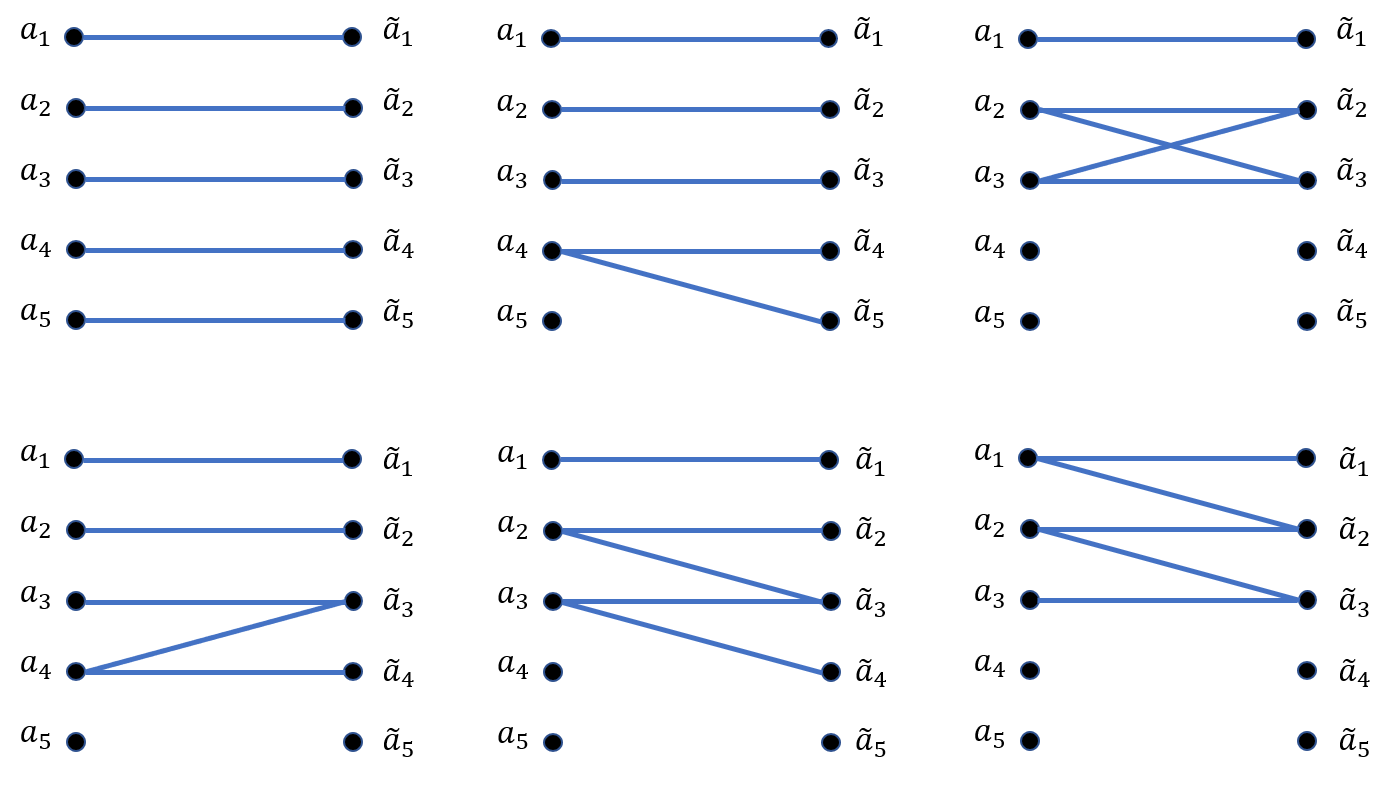
\includegraphics[width=\linewidth]{figs/Exam-BipartiteGraph.png}
\vspace*{-1cm}
\caption{辺数が5である二分グラフの例(各頂点の次数は2以下)}
\label{辺5本の場合}
\end{figure}

図\ref{辺5本の場合}のように,ある$\tilde{G}_{i}$に含まれる辺が5本であるとき,互いに隣接しない辺が3本以上存在する.
よって,補題\ref{補題14}(abc)より,$p \{x:=xy \} \preceq q_{k}$となる.
これは,仮定に矛盾する.

\textbf{(2-2)} 
$p \{ x:=ya_{i} \} \preceq q_{i}$かつ$p \{ x:=a_{i}y \} \preceq q_{i}$ $(i=1, \ldots, k-3)$とし,$p \{ x:=ya_{j+3} \} \preceq q_{j}$かつ$p \{ x:=a_{j}y \} \preceq q_{j}$ $(j=k-2,k-1)$とする.
このとき,系\ref{両方}より,$p \{ x:=a_{j+3}a_{j} \} \preceq q_{j}$となる$q_{j}$が考えられる.
よって,$\tilde{G}_{j}$には,それぞれ1本の辺が含まれる.
$G$に含まれる辺は,9本であるから,残り$9-2=7$本の辺は$\tilde{G}_{i}$ $(i=1, \ldots, k-3)$と$\tilde{G}_{k}$に含まれる.
$\tilde{G}_{i}$のいずれかに,辺が1本以上含まれる場合,$p \{ x:=ab \} \preceq q_{i}$ $(a \not = a_{i}$かつ$b \not = a_{i})$となる.
補題\ref{追加部分}より,$p \{ x:=xy \} \preceq q_{i}$となる
これは,仮定に矛盾する.
よって,$\tilde{G}_{k}$には$7$本の辺が含まれる.
ある$\tilde{G}_{i}$に含まれる辺が5本以上であるとき,互いに隣接しない辺が3本以上存在する.
補題\ref{補題14}(abc)より,$p \{x:=xy \} \preceq q_{k}$となる.
これは,仮定に矛盾する.

\textbf{(2-3)} 
$p \{ x:=ya_{i} \} \preceq q_{i}$かつ$p \{ x:=a_{i}y \} \preceq q_{i}$ $(i=1, \ldots, k-2)$とし,$p \{ x:=ya_{k+2} \} \preceq q_{k-1}$かつ$p \{ x:=a_{k-1}y \} \preceq q_{k-1}$とする.
このとき,系\ref{両方}より,$p \{ x:=a_{k+2}a_{k-1} \} \preceq q_{k-1}$となる$q_{k-1}$が考えられる.
よって,$\tilde{G}_{k-1}$には,1本の辺が含まれる.
$G$に含まれる辺は,9本であるから,残り$9-1=8$本の辺は$\tilde{G}_{i}$ $(i=1, \ldots, k-2)$と$\tilde{G}_{k}$に含まれる.
$\tilde{G}_{i}$のいずれかに,辺が1本以上含まれる場合,$p \{ x:=ab \} \preceq q_{i}$ $(a \not = a_{i}$かつ$b \not = a_{i})$となる.
補題\ref{追加部分}より,$p \{ x:=xy \} \preceq q_{i}$となる.
これは,仮定に矛盾する.
よって,$\tilde{G}_{k}$には$8$本の辺が含まれる.
ある$\tilde{G}_{i}$に含まれる辺が5本以上であるとき,互いに隣接しない辺が3本以上存在する.
補題\ref{補題14}(abc)より,$p \{x:=xy \} \preceq q_{k}$となる.
これは,仮定に矛盾する.

\textbf{(2-4)} 
$p \{ x:=ya_{i} \} \preceq q_{i}$かつ$p \{ x:=a_{i}y \} \preceq q_{i}$ $(i=1, \ldots, k-1)$とする.
$\tilde{G}_{i}$のいずれかに,辺が1本以上含まれる場合,$p \{ x:=ab \} \preceq q_{i}$ $(a \not = a_{i}$かつ$b \not = a_{i})$となる.
補題\ref{追加部分}より,$p \{ x:=xy \} \preceq q_{i}$となる.
よって,$\tilde{G}_{k}$に$9$本の辺が含まれる.
ある$\tilde{G}_{i}$に含まれる辺が5本以上であるとき,互いに隣接しない辺が3本以上存在する.
補題\ref{補題14}(abc)より,$p \{x:=xy \} \preceq q_{k}$となる.
これは,仮定に矛盾する.

\noindent\textbf{(3)}
$G^{(k-2,~k-2)}$には$4\times4=16$本の辺が含まれる.
$| A^{\prime} \cap B^{\prime} | = 0$であるとき,最大$4$つの$\tilde{G}_{i}$に辺が1本含まれ,$\tilde{G}^{(0,~0)}_{i_{0}}$と$\tilde{G}^{(0,~0)}_{i_{1}}$に,少なくとも$4 \times 4-4=12$本の辺が含まれる.
$12 > 4 \times 2 + 1$より,$\tilde{G}^{(0,~0)}_{i_{0}}$または$\tilde{G}^{(0,~0)}_{i_{1}}$は$5$本以上の辺を含む.
よって,$\tilde{G}^{(0,~0)}_{i_{0}}$または$\tilde{G}^{(0,~0)}_{i_{1}}$は,互いに隣接しない辺を3本以上含む.
したがって,補題\ref{補題14}(abc)より,$p \{x:=xy \} \preceq q_{i_{0}}$または$p \{x:=xy \} \preceq q_{i_{1}}$となる.
これは,仮定に矛盾する.  

$| A^{\prime} \cap B^{\prime} |=0$であるとき,$\tilde{G}^{(0,~0)}_{i_{0}}$と$\tilde{G}^{(0,~0)}_{i_{1}}$に含まれる辺数が最も少なくなる.
よって,$| A^{\prime} \cap B^{\prime} |=0$であるとき,矛盾であれば,$| A^{\prime} \cap B |=n$ $(n=1,2,3,4)$であるときも矛盾する.

一般化して考えていくと,$G$には$\sharp A^{\prime} \times \sharp\tilde{B}^{\prime}$本の辺が含まれる.
$| A^{\prime} \cap B^{\prime} |=0$であるとき,1本の辺を持つ$\tilde{G}^{(1,~1)}_{i_{n}}$ $(n=1,\ldots, \ell$ $(0 \le \ell \le \sharp A^{\prime}))$が最大$\sharp A^{\prime}$個存在する.
このとき,$\tilde{G}^{(0,~0)}_{j_{m}}$ $(m=1,\ldots, \sharp A^{\prime}-2)$には$\sharp A^{\prime} \times \sharp\tilde{B}^{\prime} - \ell$本の辺が含まれる.
よって,$\ell \le \sharp A^{\prime}$より,少なくとも$\sharp A^{\prime} \times \sharp\tilde{B}^{\prime} - \sharp A^{\prime}$本の辺が含まれる.
$\sharp A^{\prime}-2$個の$\tilde{G}^{(0,~0)}_{j_{m}}$に対して,合計$4(\sharp A^{\prime}-2) +1$本の辺を追加していくと,少なくとも1個のグラフは,5本以上の辺を含む.
%\begin{equation*}\label{ine}
  %\begin{split}

\begin{center}
  \begin{tabular}{l}
  $\sharp A^{\prime} \times \sharp\tilde{B}^{\prime} -\sharp A^{\prime} \ge 4(\sharp A^{\prime}-2)+1$\\
  $\sharp A^{\prime 2}-\sharp A^{\prime} \ge 4\sharp A^{\prime}-8+1$\\
%  &\sharp A^{\prime 2}-\sharp A^{\prime}-4\sharp A^{\prime}+7 \ge 0\\
  $\sharp A^{\prime 2}-5\sharp A^{\prime}+7 \ge 0$~~~~~~~~~~~~~~~~~~~~~~~~~(1)
\end{tabular}
\end{center}
  %\end{split}
  %\end{equation*}


(1)式の判別式を$D$とすると,$D=25-4\times7=-3$となる.
$D<0$より,任意の$\sharp A^{\prime}$について不等式が成り立つ.
よって,ある$\tilde{G}^{(0,~0)}_{i}$に含まれる辺は5本以上となり,互いに隣接しない辺が3本以上存在する.
したがって,補題\ref{補題14}(abc)より,$p \{x:=xy \} \preceq q_{i}$となる.
これは,仮定に矛盾する.  

以上より,$k \ge 2$においても,仮定に矛盾する.
\end{proof}

\begin{lem}[Sato et al.\cite{Sato1}]\label{補題15}
$\sharp \Sigma \ge 3$とし,$p,q$を正規パターンとする.
このとき,ある$a \in \Sigma$に対して,
$p \{ x := a \} \preceq q$かつ$p \{ x := xy \} \preceq q$ならば$p \preceq q$である.
ただし,$y$は$q$に含まれない変数記号である.
\end{lem}

%補題\ref{追加補題1},補題\ref{補題15}より,次の定理が成り立つ.

\begin{thm}\label{定理17}
$k \ge 3$,$\sharp \Sigma \ge 2k-1$,$P \in \RPatplus,Q \in \RPat^{k}$とする.
このとき,以下の{\rm (i),(ii),(iii)}は同値である.
\[
\begin{tabular}{ll}
$(\mathrm{i})$ $S_{2}(P) \subseteq L(Q),$
$(\mathrm{ii})$ $P \sqsubseteq Q,$
$(\mathrm{iii})$ $L(P) \subseteq L(Q).$
\end{tabular}
\]
\end{thm}

\begin{proof}
(ii) $\Rightarrow$ (iii)と(iii) $\Rightarrow$ (i)は自明である.
定理\ref{定理10}より,$\sharp\Sigma \ge 2k+1$のとき,(i) $\Rightarrow$ (ii)は成り立つ.
よって,$\sharp Q=k$のとき,$\sharp\Sigma = 2k-1$または$\sharp\Sigma = 2k$の場合,(i) $\Rightarrow$ (ii)が成り立つことを,$p$に含まれる変数記号の数$n$に関する数学的帰納法により証明する.

$n=0$のとき,$S_{2}(p)= \{ p \}$であり,$p \in L(Q)$となる.よって,ある$q \in Q$に対して,$p \preceq q$となる.

$n \ge 0$個の変数記号を含む任意の正規パターンに対して題意が成り立つと仮定する.
$p$を$S_{2}(p) \subseteq L(Q)$を満たす$n+1$個の変数記号を含む正規パターンとする.
$p \not \preceq q_{i}$ ($i=1, \ldots, k$)と仮定する.
$p=p_{1}xp_{2}$ ($p_{1},p_{2}$は正規パターン,$x$は変数記号),$Q=\{ q_{1}, \ldots , q_{k} \}$を考える.
$a, b \in \Sigma$に対して,$p_{a}=p \{ x := a \}$と$p_{ab}=p \{ x := ab \}$とおく.
このとき,$p_{a},p_{ab}$は$n$個の変数記号が含まれ,$S_{2}(p_{a}) \subseteq L(Q)$かつ$S_{2}(p_{ab}) \subseteq L(Q)$が成り立つことに注意する.
帰納法の仮定より,任意の$a,b \in \Sigma$に対して,$p_{a} \preceq q_{i}$かつ$p_{ab} \preceq q_{i^{\prime}}$を満たすような$i, i^{\prime} \le k$が存在する. 
$D_{i}=\{ a \in \Sigma \mid p \{ x:=a \} \preceq q_{i} \}$ \ ($i=1, \ldots, k$)とする.
ある$i$に対して,$\sharp D_{i} \ge 3$であるとき,補題\ref{補題10}より,$p \preceq q_{i}$となる.これは仮定に矛盾する.
よって,$\sharp D_{i} \le 2$ ($i=1, \ldots, k$)となる場合を考える.
$\sharp\Sigma = 2k-1$のとき,任意の$i$に対して,$\sharp D_{i}=2$または$\sharp D_{i}=1$,$\sharp\Sigma = 2k$のとき,任意の$i$に対して,$\sharp D_{i}=2$となる.
$k \ge 3$であるとき,$2k+1 \ge k+2$となる.
よって,補題\ref{追加補題1}より,$p \{ x:=xy \} \preceq q_{i}$となる$i$が存在する.
したがって,補題\ref{補題15}より,$p \preceq q_{i}$となる.
これは仮定に矛盾する.
  
以上より,(i) $\Rightarrow$ (ii)が成り立つ.
\end{proof}

この定理\ref{定理17}より,次の系が得られる.

\begin{col}\label{命題18}
$k \ge 3$,$\sharp\Sigma \ge 2k-1$,$P \in \mathcal{RP}^{+}$とする.このとき,$S_{2}(P)$は$\mathcal{RPL}^{k}$における$L(P)$の特徴集合である.
\end{col}

\begin{lem}[Sato et al.\cite{Sato1}]\label{補題19}
$\sharp\Sigma \le 2k-2$とする.このとき,$\mathcal{RP}^{k}$は包含に関するコンパクト性を持たない.
\end{lem}

\begin{proof}
$\Sigma = \{ a_{1}, \ldots , a_{k-1}, b_{1}, \ldots , b_{k-1} \}$を$(2k-2)$個の定数記号から成る集合,$p, q_{i}$を正規パターン,$w_{i}~(i = 1, \ldots , k-1)$を例\ref{例題1}と同様に定義された記号列とする.
$q_{k} = x_{1}a_{1}w_{1}xyw_{1}b_{1}x_{2}$とする.
例\ref{例題1}で示した通り,$p \{ x := a_{i} \} \preceq q_{i}$かつ$p \{ x := b_{i} \} \preceq q_{i}~(i=1,2, \ldots ,k-1)$であるとき,$S_{1}(p) \subseteq \bigcup^{k-1}_{i=1} L(q_{i})$となる. 
一方で,任意の$w$ $(|w| \ge 2)$に対して,$p \{ x:= w \} \preceq q_{k}$となる. 
すなわち,$L(p) \subseteq L(Q)$である.
しかし,$p \not \preceq q_{i}$であるため,$L(p) \not \subseteq L(q_{i}) (i=1,2, \ldots k)$である.
したがって,$\RPatkei$は包含に関するコンパクト性を持たない.
\end{proof}

定理\ref{定理17}と補題\ref{補題19}より,次の定理が成り立つ.

\begin{thm}
$k \ge 3$とし,$\sharp\Sigma \ge 2k-1$とする.
このとき,$\RPat^{k}$は包含に関してコンパクト性を持つ.
\end{thm}

$k=2$のとき,次の定理が成り立つ.

\begin{thm}\label{補題21}
$\sharp \Sigma \ge 4$とし,$P \in \RPatplus$,$Q \in \RPat^{2}$とする.
このとき,以下の{\rm (i),(ii),(iii)}は同値である.
\[
\begin{tabular}{ll}
$(\mathrm{i})$ $S_{2}(P) \subseteq L(Q),$
$(\mathrm{ii})$ $P \sqsubseteq Q,$
$(\mathrm{iii})$ $L(P) \subseteq L(Q).$
\end{tabular}
\]
\end{thm}

\begin{proof}
(ii) $\Rightarrow$ (iii)と(iii) $\Rightarrow$ (i)は自明に成り立つ.
よって,(i) $\Rightarrow$ (ii)が成り立つことを示す.
$Q= \{ q_{1}, q_{2} \}$とするとき,$p$に含まれる変数記号の数$n$に関する数学的帰納法で示す.\\
\noindent (1) $n=0$のとき,$p$は定数記号列となるので$S_{2}(p)= \{ p \}$となり
(i)より,$p \in L(Q)$となる.
よって,ある$q \in Q$に対して$p \preceq q$となる.\\
\noindent (2) $n=k$個の変数記号を含むすべての正規パターンに対して有効であると仮定する.
そして,$p$を$S_{2}(p) \subseteq L(Q)$を満たす$(n+1)$個の変数記号を含む正規パターンとする.

$p \not \preceq q_{i}$ ($i=1, 2$)と仮定する.
$p=p_{1}xp_{2}$ ($p_{1}, p_{2}$は正規パターン,$x$は変数記号)を考える.
$a, b \in \Sigma$に対して,$p_{a}=p \{ x := a \}$,$p_{ab}=p \{ x := ab \}$とおく.
このとき,$p_{a},p_{ab}$は$n$個の変数記号が含まれ,$S_{2}(p_{a}) \subseteq L(Q)$,$S_{2}(p_{ab}) \subseteq L(Q)$が成り立つことに注意する.
帰納法の仮定より,任意の$a, b \in \Sigma$に対して,$p_{a} \preceq q_{i}, p_{ab} \preceq q_{i^{\prime}}$を満たすような$i, i^{\prime} \le k$が存在する.

ある$i$に対して$\sharp D_{i} \ge 3$のとき,補題\ref{補題10}より,$p \preceq q_{i}$となる.
よって,任意の$i$に対して,$\sharp D_{i} \le 2$となる.
したがって,$\sharp D_{1}=2$かつ$\sharp D_{2}=2$となる場合を考える.

$\sharp \Sigma = k+2$であるとき,$k=2$より,$\sharp \Sigma =4$となる.
よって,補題\ref{追加補題1}より,ある$i$に対して,$p \{ x:=xy \} \preceq q_{i}$となる.
したがって,補題\ref{補題15}より,$p \preceq q_{i}$となる.
これは,仮定に矛盾する.

以上より,(i) $\Rightarrow$ (ii)が成り立つ.
\end{proof}

次の例は,$k = 2$における定理\ref{補題21}の反例である.
\begin{ex}\label{反例thm17}
$\Sigma= \{a, b, c \}$を$3$つの定数記号から成る集合,$p,q_{1},q_{2}$を正規パターン,$x,x^{\prime},x^{\prime\prime}$を変数記号とする.
\begin{eqnarray*}
p = x^{\prime}axbx^{\prime\prime},
q_{1} = x^{\prime}abx^{\prime\prime},
q_{2} = x^{\prime}cx^{\prime\prime}.
\end{eqnarray*}
$w \in \Sigma^{+}$とする.$w$に$c$が含まれるとき,$p \{ x:=w \} \preceq q_{2}$となり,$c$が含まれないとき,$p \{ x:=w \} \preceq q_{1}$となる.
よって,$L(p) \subseteq L(q_{1}) \cup L(q_{2})$である.
しかし,$p \not \preceq q_{1}$かつ$p \not \preceq q_{2}$である.
\end{ex}

定理\ref{補題21}より,次の2つの系が成り立つ.
\begin{col}
$\sharp\Sigma \ge 4$とし,$P \in \RPatplus$とする.
このとき,$S_{2}(P)$は,$\RPatL^{2}$における$L(P)$の特徴集合である.
\end{col}

\begin{col}
$\sharp\Sigma \ge 4$とする.このとき,クラス$\mathcal{RP}^{2}$は包含に関してコンパクト性を持つ.
\end{col}

